\documentclass[addpoints]{exam}
% \documentclass[addpoints,12pt]{exam}

\usepackage[slovene]{babel}
\usepackage{amsfonts}
\usepackage{amssymb}
\usepackage{amsmath}
\usepackage{float}
\usepackage{graphicx}
\usepackage{enumitem}
\usepackage{color}
\usepackage{eurosym}

\usepackage{pgfpages}
% \usepackage{tikz}
\usepackage{wrapfig}
\usepackage{pgfkeys}
\usepackage{pgfplots}
\usepackage{xcolor}
\usepackage{tkz-euclide}
\usepackage{xfp}




%Komentar naslednje vrstice glede na verzijo testa -- rešitve ali prostor za odgovore:
% \printanswers

% \linespread{2}


\pointsinrightmargin
\marginbonuspointname{}


\renewcommand{\solutiontitle}{\noindent\textbf{Rešitve in točkovanje:}\par\noindent}

\colorgrids
\definecolor{GridColor}{gray}{0.7}
\setlength{\gridsize}{7mm}

\extrawidth{5mm}
\setlength{\rightpointsmargin}{1.5cm}

\begin{document}

\runningfooter{}{}{}

\begin{center}
    \fbox{\fbox{\parbox{15cm}{\centering
    Tretje pisno preverjanje znanja \\ 2. letnik \\ marec 2026 \\ (Potence in koreni; Funkcija; Potenčna funkcija; Korenska funkcija)}}}
\end{center}

\vspace{0.1in}
\makebox[\textwidth]{Ime in priimek, oddelek:\enspace\hrulefill}


\begin{center}
    \chqword{Naloga}
    \chpword{Možne točke}
    \chbpword{Dodatne točke}
    \chsword{Dosežene točke}
    \chtword{Skupaj}  
    \combinedpointtable[h][questions]
    % \combinedgradetable[h][questions]

\end{center}

\vspace{0.1in}


\begin{questions}

    % 1. vprašanje

    \question[7]
    Izračunajte natančno vrednost izraza. 
    $$ \left(3\dfrac{3}{8}\right)^{\frac{2}{3}}\cdot 0.25^{-0.5}\cdot \left(3-\sqrt{5}\right)\sqrt{7+3\sqrt{5}} - \sqrt[3]{10^2+0.2^{-2}} $$

    % \begin{solution}[8cm]
       
    % \end{solution}


    % 2. vprašanje

    \question[6]
    Rešite enačbo. 
    $$ \sqrt{x+3+\sqrt{x+2}}=\sqrt{3} $$

    % \begin{solution}[5.25cm]
       
    % \end{solution}


% \newpage
    % 3. vprašanje

    \question
    Dana je funkcija $f(x)=\left(x-2\right)^{2}-1$.

    \begin{parts}
        \part[2]
        Zapišite definicijsko območje $D_f$ in zalogo vrednosti $Z_f$ funkcije $f$. 

            % \begin{solution}[1.5cm]

            % \end{solution}
        
        \part[4] 
        Izračunajte ničle in začetno vrednost funkcije $f$.
    
            % \begin{solution}[6cm]

            % \end{solution}

        \part[2] 
        Računsko preverite, ali je funkcija $f$ soda ali liha.
    
            % \begin{solution}[5cm]

            % \end{solution}

        \part[3] 
        Določite presečišča grafa funkcije $f$ s premico $y=-1$.
    
            % \begin{solution}[4cm]

            % \end{solution}

        \part[3]
        Določite inverzno funkcijo $f^{-1}$ funkcije $f$.

            % \begin{solution}[5cm]

            % \end{solution}
            

        \part[5] 
        Narišite graf funkcije $f$.
    
            % \begin{solution}[5cm]

            % \end{solution}

    \end{parts}


    

    % \newpage
    % 4. vprašanje

    \question
    Na sliki je graf funkcije $g$, ki smo ga dobili s transformacijo grafa funkcije $f(x)=\sqrt[3]{x}$.
    
    \begin{figure}[H]
        \centering
        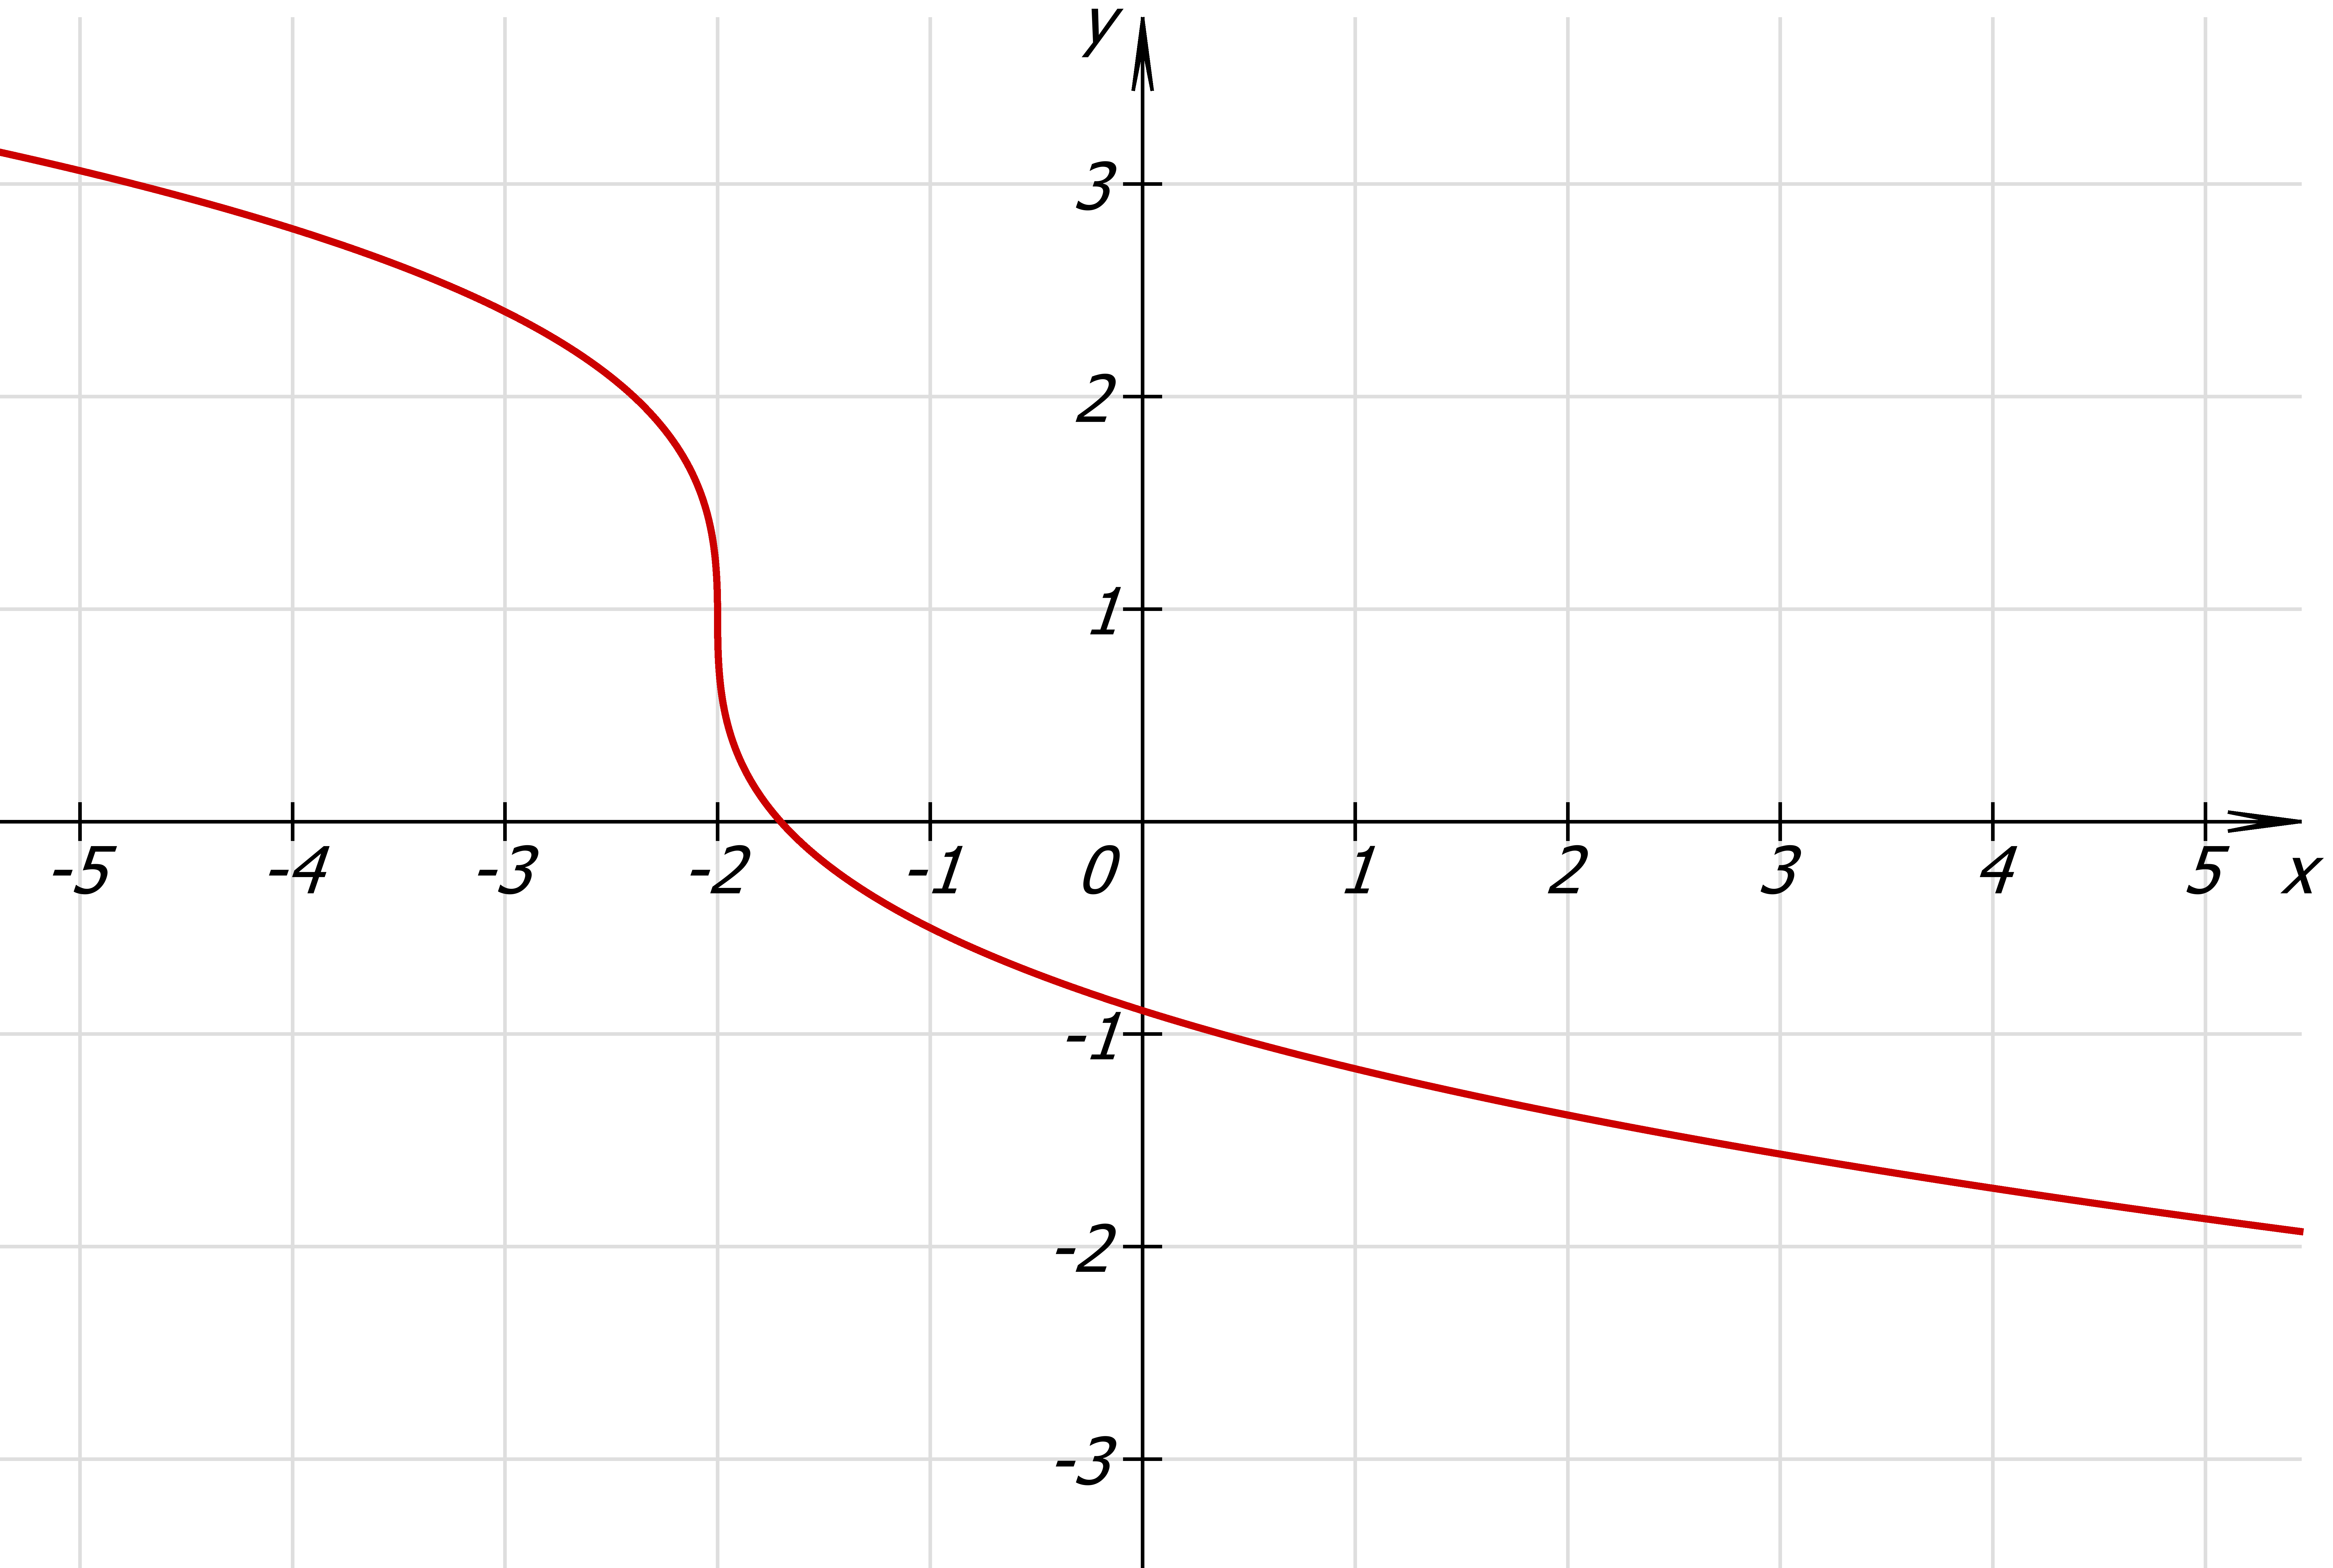
\includegraphics[scale=0.05]{preverjanje3_korenska.png}
    \end{figure}

    \begin{parts}
        \part[2] 
        Na zgornjo sliko dorišite graf funkcije $h(x)= -g(x)$.
        
            % \begin{solution}

            % \end{solution}        

        \part[4]
        Zapišite predpis funkcije $g$, če njen graf poteka skozi točko $(6,-2)$.

            % \begin{solution}[7cm]

            % \end{solution}

    
        \part[4]
        Določite inverzno funkcijo $i^{-1}$ funkciji $i(x)=-2 f(3x+3) + 3$.
        
            % \begin{solution}[5cm]

            % \end{solution}


    \end{parts}





\end{questions}



\end{document}